\documentclass[tikz,border=3mm]{standalone}
\usepackage[T1]{fontenc}
\usepackage{lmodern,amsmath,amssymb}
\usetikzlibrary{arrows.meta,calc,positioning,fit,backgrounds}
\definecolor{accent}{RGB}{36,91,158}
\definecolor{soft}{RGB}{225,237,248}
\definecolor{muted}{RGB}{122,134,145}
\definecolor{warm}{RGB}{250,242,220}
\tikzset{every node/.style={font=\sffamily\small},
vertex/.style={circle,draw=black!80,fill=white,minimum size=7.5mm,inner sep=1pt},
edge/.style={draw=accent!55,line width=.65pt},
highlight/.style={draw=accent,line width=1.7pt},
box/.style={draw=accent!70,rounded corners=2pt,fill=soft!45,align=center,inner sep=6pt},
heading/.style={font=\sffamily\bfseries\normalsize,align=center},
map/.style={-{Stealth[length=2mm]},line width=.8pt},
}
\hyphenpenalty=10000\exhyphenpenalty=10000
\begin{document}
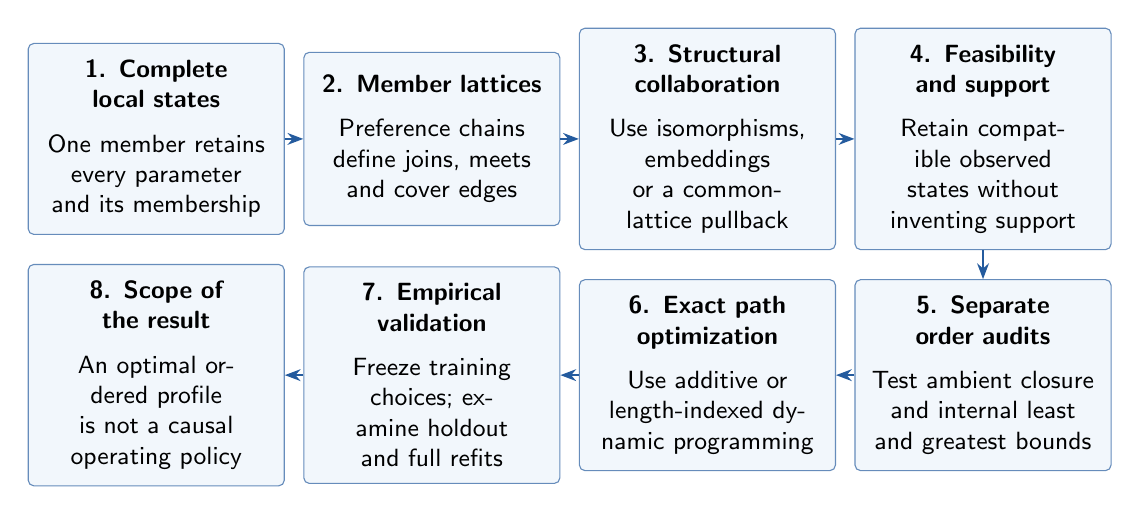
\begin{tikzpicture}[x=1cm,y=1cm]
\node[box,text width=2.83cm,minimum height=2.20cm] (b0) at (0.0,3) {\textbf{1. Complete local states}\\[5pt]One member retains every parameter and its membership};
\node[box,text width=2.83cm,minimum height=2.20cm] (b1) at (3.5,3) {\textbf{2. Member lattices}\\[5pt]Preference chains define joins, meets and cover edges};
\node[box,text width=2.83cm,minimum height=2.20cm] (b2) at (7.0,3) {\textbf{3. Structural collaboration}\\[5pt]Use isomorphisms, embeddings or a common-lattice pullback};
\node[box,text width=2.83cm,minimum height=2.20cm] (b3) at (10.5,3) {\textbf{4. Feasibility and support}\\[5pt]Retain compatible observed states without inventing support};
\node[box,text width=2.83cm,minimum height=2.20cm] (b4) at (10.5,0) {\textbf{5. Separate order audits}\\[5pt]Test ambient closure and internal least and greatest bounds};
\node[box,text width=2.83cm,minimum height=2.20cm] (b5) at (7.0,0) {\textbf{6. Exact path optimization}\\[5pt]Use additive or length-indexed dynamic programming};
\node[box,text width=2.83cm,minimum height=2.20cm] (b6) at (3.5,0) {\textbf{7. Empirical validation}\\[5pt]Freeze training choices; examine holdout and full refits};
\node[box,text width=2.83cm,minimum height=2.20cm] (b7) at (0.0,0) {\textbf{8. Scope of the result}\\[5pt]An optimal ordered profile is not a causal operating policy};
\draw[map,draw=accent] (b0) -- (b1);
\draw[map,draw=accent] (b1) -- (b2);
\draw[map,draw=accent] (b2) -- (b3);
\draw[map,draw=accent] (b3) -- (b4);
\draw[map,draw=accent] (b4) -- (b5);
\draw[map,draw=accent] (b5) -- (b6);
\draw[map,draw=accent] (b6) -- (b7);
\end{tikzpicture}
\end{document}
